% REMEMBER: You must not plagiarise anything in your report. Be extremely careful.

\documentclass{l4proj}
\usepackage{graphicx}
\usepackage{float}
\usepackage{wrapfig}
\graphicspath{ {./images/} }
    
%
% put any additional packages here
%
\newcommand{\jake}[1]{\marginpar {\footnotesize \color{red} {\bf JL:} \textsf{#1}}}

\begin{document}

%==============================================================================
%% METADATA
\title{Extracting Relations between Chemicals and Genes from Biomedical Literature}
\author{Chlo\"e Smart}
\date{24th of March, 2023}

\maketitle

%==============================================================================
%% ABSTRACT
\begin{abstract}
    Manually processing an abundance of biomedical text can prove to be extremely costly and inefficient, and often causes bottlenecks within the processes of drug discovery, design and re-purposing. Employing the use of transformer models to automate these processes has become crucial to solving these problems, however there are some improvements that can be made to make them more effective. This project attempts to investigate particular research questions that may elucidate some of the processes behind deep learning methods for supervised relation extraction, with a focus on relations between chemicals and genes. Prior experiments regarding relation extraction explored adjusting the structure of input sentences, the types of output sentence representations, the structure of the model and different regularisation methods in order to improve relation predictions. These methods were then applied to the biomedical domain to observe their effectiveness on a more complex input structure. 
    
    It was found that adjusting the input text structure and extracting entity specific sentence representations, specifically tagging entities and using their tags for classification, was significantly more effective than using the standard [CLS] representation, almost doubling classification performance. Furthermore, there was an investigation into the amount of entity information that was necessary in order for the model to be able to learn entity relationships, and it was revealed that replacing entity mentions with just their type significantly reduced the complexity of the input and therefore improved results by over 10\%. There was also an inquiry into the optimal amount of dropout required to make the model more generalisable without any performance degradation. It was found that the best dropout probability was dependent on the type of sentence representations being used, with dropout 0.5 being best for entity representations and 0.6 being best for [CLS] representations. 
    
    Finally, the model was optimised using grid search in order to find the best parameters for the input data, which improved performance by a further 10\%. The results for each research question were then combined to obtain the best F1 score on the test set, which was 78\%. The best relation-specific F1 score was 90\% for the PART-OF relation. These results can be used to improve the reliability of models used for relation extraction in the biomedical domain.
    
\end{abstract}

%==============================================================================

% EDUCATION REUSE CONSENT FORM
% If you consent to your project being shown to future students for educational purposes
% then insert your name and the date below to  sign the education use form that appears in the front of the document. 
% You must explicitly give consent if you wish to do so.
% If you sign, your project may be included in the Hall of Fame if it scores particularly highly.
%
% Please note that you are under no obligation to sign 
% this declaration, but doing so would help future students.
%
\def\consentname {Chlo\"e Smart} % your full name
\def\consentdate {24th March 2023} % the date you agree
%
\educationalconsent


%==============================================================================
\tableofcontents

%==============================================================================
%% Notes on formatting
%==============================================================================
% The first page, abstract and table of contents are numbered using Roman numerals and are not
% included in the page count. 
%
% From now on pages are numbered
% using Arabic numerals. Therefore, immediately after the first call to \chapter we need the call
% \pagenumbering{arabic} and this should be called once only in the document. 
%
% Do not alter the bibliography style.
%
% The first Chapter should then be on page 1. You are allowed 40 pages for a 40 credit project and 30 pages for a 
% 20 credit report. This includes everything numbered in Arabic numerals (excluding front matter) up
% to but excluding the appendices and bibliography.
%
% You must not alter text size (it is currently 10pt) or alter margins or spacing.
%
%
%==================================================================================================================================
%
% IMPORTANT
% The chapter headings here are **suggestions**. You don't have to follow this model if
% it doesn't fit your project. Every project should have an introduction and conclusion,
% however. 
%
%==================================================================================================================================
\chapter{Introduction}
%Why should the reader care about what are you doing and what are you actually doing?
%Motivate first, then state the general problem clearly.

% reset page numbering. Don't remove this!
\pagenumbering{arabic} 

\section{Motivation}
There is a plethora of unstructured data that exists in the wild, including log files, social media posts, emails and research documents. As technology becomes more sophisticated, it becomes essential for machines to contextualise this information and create a structure that can assist in performing specified tasks. This is particularly important in bio-medicine, where the goal is designing and re-purposing drugs to find disease treatments. Publications within the biomedical domain differ greatly from literature produced in other domains since they contain technical terms and abbreviations specific to the field and may require specialised knowledge to be understood. These publications are also heterogeneous, covering many sub-disciplines such as pharmacology and genetics.

In order to develop a drug, a large amount of research is required to determine the relationships of biomedical entities, such as interactions between particular chemicals and proteins. This consists of several researchers having to scour through thousands of biomedical documents, interpret the semantics of these papers, and manually input data about how several entities are related. As the number of biomedical publications exponentially increases, these processes become significantly more time-consuming and expensive, causing extreme bottlenecks in drug discovery and design processes. A solution to this problem is to develop a system that can read thousands of text documents and automatically detect relations between entities. 
\\ \\
These models have been proven to be incredibly effective at relation extraction, which is extracting semantic relationships from a set of entities that occur within text. This is because they can capture complex text semantics and detect subtle relationships between entities. Despite their benefits, it is difficult for researchers to explain how they produce particular results. An increasingly popular approach to this problem is to produce a system that employs deep learning. This project aims to explore the nuances behind how transformer models interpret input data and learn from it, including altering the structure of the input data, extracting different sentence representations from the output data, and performing regularisation. It will focus on extracting chemical-protein relations within an annotated biomedical text corpus.

\newpage
\section{Aims}
The aim is to explore the effectiveness of using different techniques on a deep learning model in order to extract chemical-gene relations from biomedical literature. In order for this to be achieved, the following criteria must be met:
\begin{itemize}
    \item Observe and describe existing approaches of using deep learning for relation extraction, and highlight any particular concepts that are worth further investigation. (Section 2)
    \item Propose a set of research questions to investigate and justify why they have been chosen (Section 3) 
    \item Describe the structure of the dataset, implementation and design details that will be included within the investigation of these research questions. (Section 4)
    \item Evaluate neural network performance for each research question using standard classification metrics, and explore the performance for different architecture variants and regularisation methods. (Section 5)
    \item Discuss modifications that can be made to optimize the model and observe the effects of combining all research results together (Section 6) 
    \item Explore the limitations of the approach to the research and propose potential future projects that can enhance model performance. (Section 7)
\end{itemize}

%==================================================================================================================================
\chapter{Background}
%What did other people do, and how is it relevant to what you want to do?
%Don’t give a laundry list of references.
%Tie everything you say to your problem.
%Present an argument.
%Think critically; weigh up the contribution of the background and put it in context.
%Don’t write a tutorial; provide background and cite references for further information

%\section{Introduction}
%This section introduces the concept of relation extraction, and how modern approaches typically utilise transformer models, and how they are typically used within different methods of biomedical relation extraction. It then goes on to explore specific implementations of chemical-protein relation extraction, and highlights key methods that can be analysed further.
% Change this once section is written

\section{Relation Extraction}
Relation extraction is the process of extracting semantic relationships from a set of entities that typically occur within text. These can occur between two or more entities, and the relationships in question can be of multiple types. We can elucidate this concept with an example sentence:

\begin{figure}[h]
    \centering
    \fbox{\begin{minipage}{30em}
\centering
“\textbf{Paris} is the capital of \textbf{France}.”
\end{minipage}}
  \caption{Example sentence in which to determine a relation.}
  \label{fig:Tagging}
\end{figure}


In this case, we have entities "Paris" and "France", and we wish to determine the relationship between them given the context of the rest of the sentence. This sentence determines a "capital\_of" relation between these two entities, which can be represented using the triple (Paris, capital\_of, France). For our specific problem, we will be determining relations between biomedical entities, which tend to be less atomic when compared to entities in other domains, and therefore can be more challenging to detect and analyse within text. Several relation extraction methods can be used with transformer models to establish these entity relationships.

\cite{comparison} explored relation extraction within the biomedical domain, focusing on extracting relations between chemical and protein entities. They conducted research comparing three methods of chemical-protein relation extraction on biomedical text, including rule-based, machine learning and deep learning. The performance of fine-tuned transformer models outperformed all other approaches, with one BERT model producing an F1 score of 92\% compared with figures of around 80\% for their rule-based and machine-learning approaches. They found a particular benefit in using transformer models since they were more resilient to small and imbalanced datasets, likely due to their extensive pre-training on large amounts of data a priori. This could be useful when dealing with data within the biomedical domain since some common diseases might be more saturated with literature than rare diseases, so it is important to successfully extract relations for these papers despite their imbalance.

\subsection{Supervised}
Supervised relation extraction takes several text features as input, including tokens, Named Entity Recognition (NER) tags and context words. The relevance of particular data to a specific relation type is often manually labelled, in addition to if sentences contain a relevant relation. A classifier is then trained to learn the relevance of particular sentences and is used to predict relations in new text data. Upon their research into different relation extraction methods, \cite{supervised} recognised that using supervised approaches for tasks within a restricted domain was often the most effective compared to other methodologies.
\\
Within the context of biomedical text mining, there are several patterns that researchers try to identify in order to determine information about particular biomedical entities. Using a large corpus of biomedical text can provide high-quality information regarding the relations between these entities, allowing for explicit negative examples during training. Within their paper, \cite{supervised} used the example of cancer researchers using inferences like "Gene X with mutation Y leads to malignancy Z" to isolate cancerous genes. It is worth noting that this paper is quite dated regarding its information, and therefore there isn't a thorough analysis of more modern methods of relation extraction, such as using transformer models. Despite this, it provides an insight into why supervised relation extraction is often desired when extracting relations from biomedical literature.

\section{Transformer Models}
Transformers are deep learning models that are designed to process sequential input data using the concept of self-attention. In self-attention, the model calculates weights for each element in the input sequence based on its importance for creating a representative context vector. Within recent years, there are several instances of transformer models that have been investigated, each with their own specialisms and functionalities. The Bidirectional Encoder Representations from Transformers (BERT) model was devised by \cite{BERT} to pre-train bidirectional representations from text, achieved by joint conditioning on both left and right context throughout all layers. This differs from previous transformer models, which typically looked at a text sequence from left to right or combined left-to-right and right-to-left training.

In their paper, BERT was tested with the General Language Understanding Evaluation (GLUE) benchmark, a collection of several natural language understanding (NLU) tasks used to evaluate machine learning model performance in natural language comprehension. These tasks include sentiment analysis, question answering and natural language inference. When compared against previous state-of-the-art transformer models such as GPT and ELMo, BERT experienced an average accuracy improvement of 4.5\%. Using BERT for biomedical relation extraction is, therefore, more likely to yield promising results than using other transformers since it can learn more from the context of each sentence.

\begin{figure}[!htb]
    \centering
    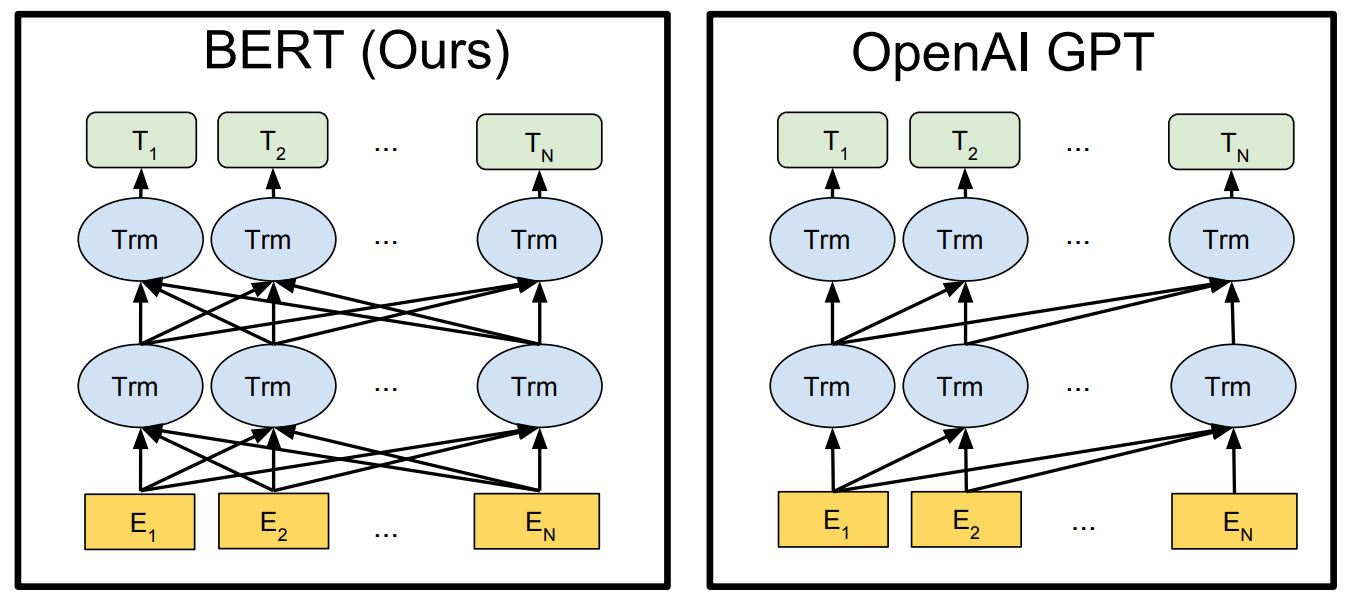
\includegraphics[width=14cm]{images/BERTvsGPT.png}
  \caption{Figure from the BERT paper (\cite{BERT}) illustrating the differences in pre-training model architectures. BERT uses a bidirectional Transformer. OpenAI GPT uses a left-to-right Transformer. Only BERT representations are jointly conditioned on both left and right context in all layers.}
  \label{fig:BERTvsGPT}
\end{figure}

\newpage
\section{Feature Extraction}
One of the ways in which the task of relation extraction can be represented is with text classification. Text classification involves dividing the input text into fragments and classifying these fragments based on a set of pre-defined categories. In biomedical relation extraction, this typically involves splitting the text into sentences, assigning labels based on which relations can be observed within the sentence, and training a model with these inputs. This can allow the model to learn patterns about which semantics represent particular relations, allowing them to predict the existence of relations within unseen sentences.

Feature extraction is the idea of extracting meaningful values derived from raw data that can be used in downstream tasks such as classification or regression. \cite{logreg} utilised BERT feature extraction with logistic regression within their own research, which involved sentence-level classification to detect propaganda within text. This involved using a pre-trained BERT model to obtain features about the text category and then classifying the features using Logistic regression. They obtained the best results by creating a model that considers additional features of the text as input, such as the length of the text and the level of positive and negative words within the text. This paper could have gone into more detail regarding the extent to which logistic regression was the superior model to use in conjunction with BERT, just that it appeared to have better performance than other models that they tested. Their use of additional features to enhance their model for their specific task can be applied to the biomedical domain, where particular textual characteristics provide more information regarding the nature of the relations within text. Figure \ref{fig:Feature} shows an example of using feature extraction using both BERT and logistic regression models.

\begin{figure}[htb]
    \centering
    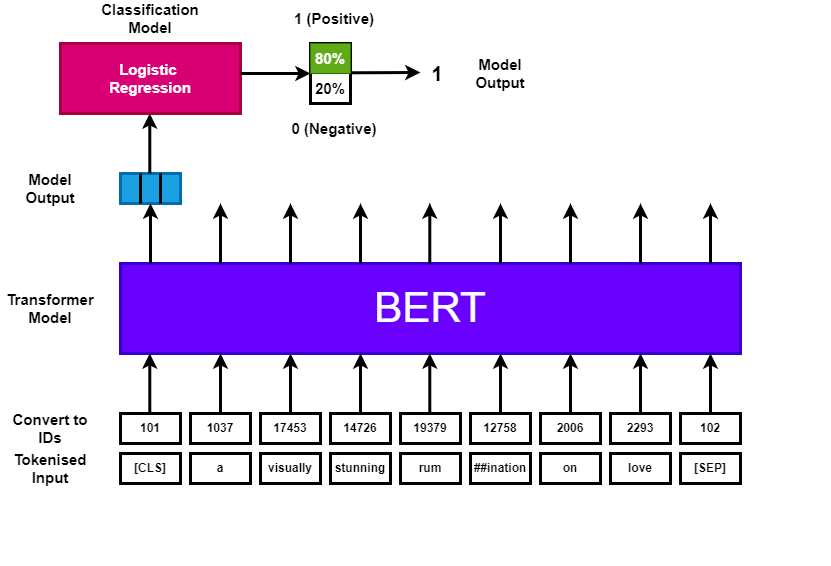
\includegraphics[width=14cm]{images/Feature.png}
  \caption{Feature Extraction Demonstration. The sentence is converted to IDs and processed through a BERT model. The embeddings for the [CLS] tag are then used as input into the Logistic Regression model to be classified.}
  \label{fig:Feature}
\end{figure}

\subsection{Pre-trained BERT Models}
BERT can be altered depending on the task that it is used for, such as pre-training and fine-tuning specific types of data. When it comes to biomedical documents, there is a change in word distribution that often causes generalised models such as BERT to perform poorly. It is usually more beneficial to pre-train BERT using biomedical documents to familiarise it with words and abbreviations specific to this domain. \cite{BioBERT} devised BioBERT, a model pre-trained using general-domain text, in addition to millions of in-domain PubMed documents. Compared with BERT, they experienced a 0.62\% F-Score improvement in named entity recognition (NER), 2.80\% F-Score improvement in their chemical-protein relation extraction task, and a 12.24\% MRR improvement in question answering.

A commonly held assumption is that the more text BERT is pre-trained on, the more beneficial the resultant model will be. \cite{PubMedBERT} attempted to challenge this assumption by creating a model called PubMedBERT, which was pre-trained solely on PubMed articles. In the paper, they point out how their method of domain-specific pre-training from scratch ensured that biomedical entities could be recognised in full, whilst other models using out-domain vocabulary tended to split the words into irrelevant subwords during tokenisation. 

\begin{figure}[hbt!]
    \centering
    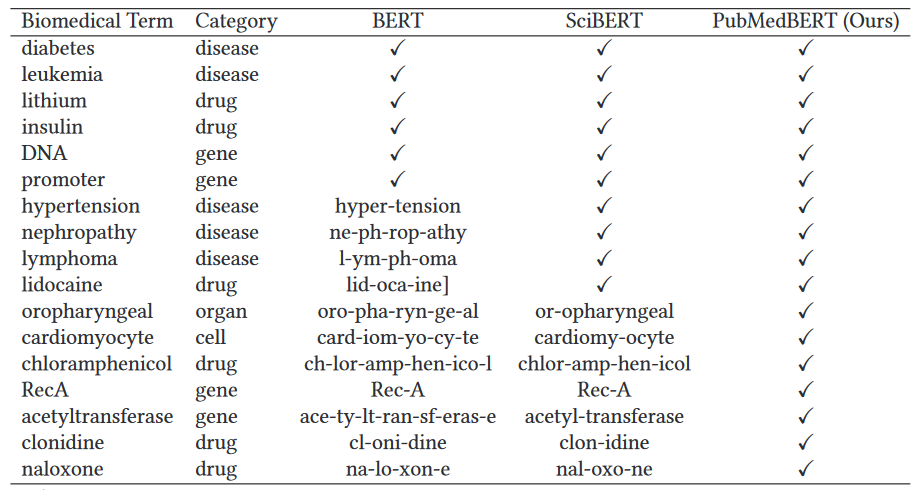
\includegraphics[width=14cm]{images/PubMedBERT.png}
  \caption{Figure from the PubMedBERT paper written by \cite{PubMedBERT} that demonstrates that the entire words for biomedical terms are preserved post-tokenisation}
  \label{fig:BERTvsGPT}
\end{figure}

When compared against the BLURB benchmark for biomedical NLP, PubMedBERT had a marginal improvement over BioBERT (0.82\%); however, there was no extensive comparison between these two models. It is clear that having some semblance of domain-specific pre-training, regardless of whether or not it is in conjunction with general-domain text, can cause a significant improvement in the results of various biomedical tasks. Using one of these models will likely provide more context within biomedical literature, making it more likely for BERT's self-attention mechanism to interpret the significance of biomedical entities correctly and, therefore, more accurately deduce relations within text.

\newpage
\section{Sentence Representations}
\cite{architectures} investigated a method of generalised relation extraction called 'Matching the blanks', which involved training a transformer model without any supervision from a knowledge graph or human annotators. Within their implementation, they explored different ways text input can be structured to affect a transformer model's interpretation. They had two queries in mind - how to \textbf{represent entities of interest} in the input to BERT, and how to \textbf{extract a fixed length representation} of a relation from BERT's output. For the first query, they investigated altering the 'Standard' input - using [CLS] and [SEP] tags to indicate the beginning and ends of sentences, as demonstrated in figure \ref{fig:Standard}. 

\begin{figure}[htb]
    \centering
   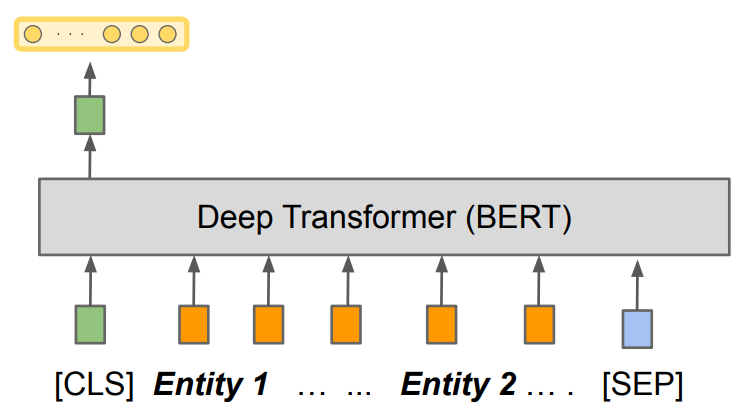
\includegraphics[width=10cm]{images/Standard.png}
  \caption{Standard input sentence with standard sentence representation ([CLS])}
  \label{fig:Standard}
\end{figure}

To address the 'Standard' representation's lack of explicit entity identification, they introduced a 'Positional Embedding' input. Different segmentation embeddings are added to each token depending on which part of the sentence they relate to. They then compared these to an 'Entity Marker' input, where they add tokens marking the beginning and end of entities within the sentence, as illustrated in figure \ref{fig:EMCLS}. 

\begin{figure}[htb]
    \centering
   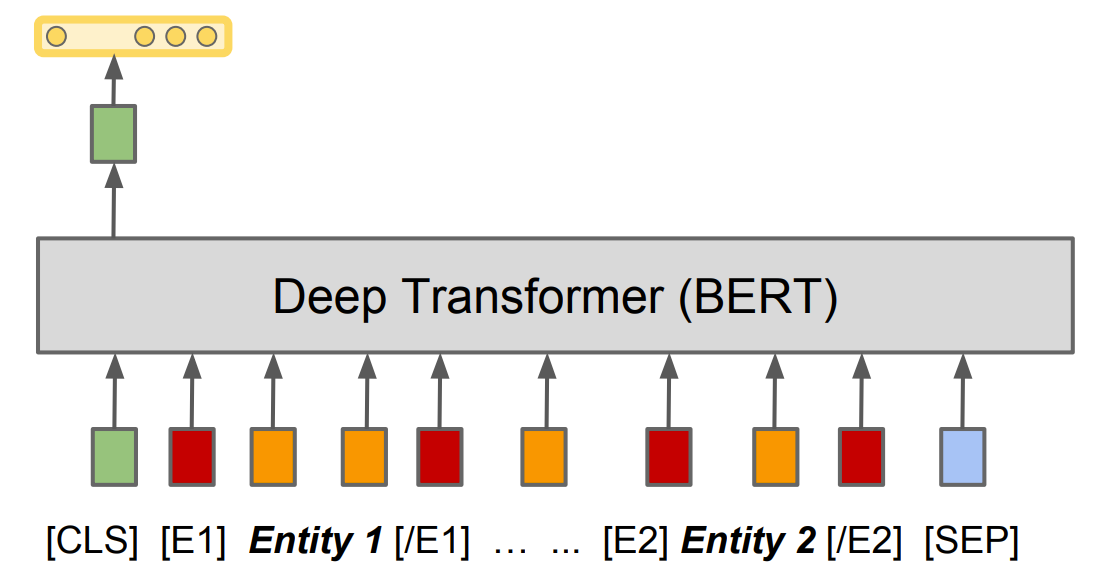
\includegraphics[width=10cm]{images/EMCLS.png}
  \caption{Entity Marker input sentence with standard sentence representation ([CLS])}
  \label{fig:EMCLS}
\end{figure}

For the second query, they explored three methods of extracting fixed-length representations from BERT's output, including the standard method of extracting the [CLS] token (figure \ref{fig:EMCLS}) expressed by \cite{BERT}, concatenating embedding representations of every token representing an entity name (mention pooling) as seen in figure \ref{fig:Ment}, and finally concatenating embedding representations of the entity start markers appearing within the 'Entity Marker' architecture shown in figure \ref{fig:EMES}.

\begin{figure}[htb]
    \centering
    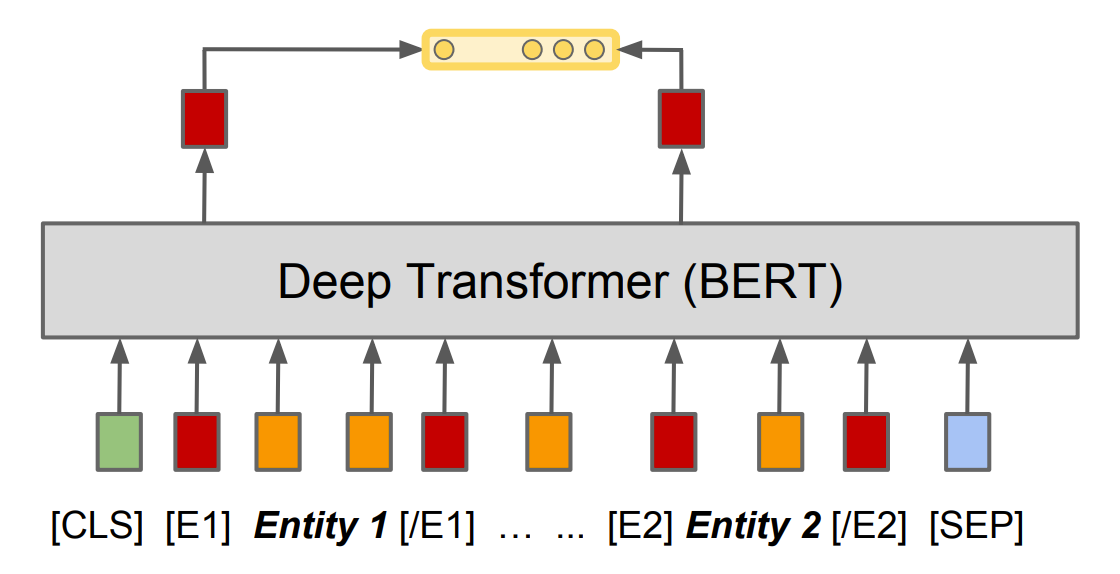
\includegraphics[width=10cm]{images/EMES.png}
  \caption{Entity Marker input sentence with Entity marker representation ([E1]/[E2])}
  \label{fig:EMES}
\end{figure}

\begin{figure}[htb]
    \centering
   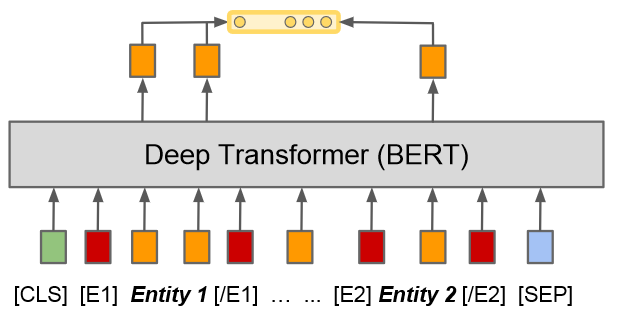
\includegraphics[width=10cm]{images/Ment.png}
  \caption{Entity Marker input sentence with Mention pooling representation}
  \label{fig:Ment}
\end{figure}

Using the' Entity Marker' architecture, they experienced the best scores for any embedding extraction. Compared to the other sentence inputs, there was a significant difference in the F1-score across all datasets of around 20\%. The best sentence representation from this architecture was the concatenation of entity markers, which improved the [CLS] representation by around 10\%. They determined that providing positional information is "critical for the model to learn useful relation representations". For their 'Matching the Blanks' task, \cite{architectures} used a dataset focused on generalised relation extraction. Using these architectures with a focus on the biomedical domain could be extremely valuable, particularly since the vast majority of implementations for biomedical relation extraction typically focus on extracting representations from [CLS] tags and do not explore other fixed-length representations from BERT's output.

\section{Entity Tagging}
Entity tagging is typically used within deep learning to provide BERT with more context regarding what it should pay attention to during training. Entity marking was demonstrated in the above example, where markers determine the location of each desired entity within the text without losing the context of the entity mention, whilst entity masking is replacing the names of relevant entities with a singular tag representation. 

\cite{mask} investigated how much information about entity mentions is required for BERT to learn more accurate patterns during training in classifying news articles. Figure \ref{fig:TACRED} is an example sentence from the TACRED dataset, which is used for their news classification task and will be used to compare each approach. 

\begin{figure}[h]
    \centering
    \fbox{\begin{minipage}{30em}
\centering
Dozens of lightly regulated subprime lenders, including New Century Financial Corp., have failed and troubled \textbf{Countrywide Financial Corp.} which was acquired by \textbf{Bank of America Corp}
\end{minipage}}
  \caption{Example sentence from the TACRED dataset. The subject being analysed in this case is Countrywide Financial Corp, and the object is Bank of America Corp.}
  \label{fig:TACRED}
\end{figure}

They first tested providing both the context of the sentence and the entity mention within the input. They used entity markers at the beginning and end of the entity mentions to identify the entities of interest. This can be observed in figure \ref{fig:TACREDmark}, where the example sentence is adapted with entity markers:

\begin{figure}[h]
    \centering
    \fbox{\begin{minipage}{30em}
\centering
Dozens of lightly regulated subprime lenders, including New Century Financial Corp., have failed and troubled \textbf{[E1] Countrywide Financial Corp. [/E1]} which was acquired by \textbf{[E2] Bank of America Corp [/E2]}
\end{minipage}}
  \caption{Example sentence representing the sentence with both context and entity mentions}
  \label{fig:TACREDmark}
\end{figure}

Next, they decided to create an input that specifies the type of each entity mention in addition to their surrounding context, as shown in figure \ref{fig:TACREDsmask}

\begin{figure}[h]
    \centering
    \fbox{\begin{minipage}{30em}
\centering
Dozens of lightly regulated subprime lenders, including New Century Financial Corp., have failed and troubled \textbf{[organization]} which was acquired by \textbf{[organization]}
\end{minipage}}
  \caption{Example sentence with masks representing the entity types. In this case, both entities are organisations.}
  \label{fig:TACREDsmask}
\end{figure}

Finally, they investigated omitting all information about the entity mentions altogether, leaving just the sentence context for the transformer models to learn from, as shown in figure \ref{fig:TACREDgmask}.

\begin{figure}[htb]
    \centering
    \fbox{\begin{minipage}{30em}
\centering
Dozens of lightly regulated subprime lenders, including New Century Financial Corp., have failed and troubled \textbf{[SUBJ]} which was acquired by \textbf{[OBJ]}
\end{minipage}}
  \caption{Example sentence where all entity information is omitted.}
  \label{fig:TACREDgmask}
\end{figure}


They tested these inputs for BERT and with the addition of the Matching the Blanks model suggested by \cite{architectures}. They discovered that providing context and highlighting entity mentions provided the most optimal results, suggesting that BERT relies on all information about entity mentions to make the best decisions. They also performed tests omitting the context of each sentence and only providing the different entity formats specified above. They discovered that BERT gains a lot of information from the type of entity specified within the text. One of the conclusions stated by \cite{mask} was that existing RE datasets might leak superficial cues through entity mentions, and models may not be able to understand context as expected. Performing analysis on entity marking and masking methods within the context of biomedical relation extraction could provide researchers with more information regarding how best to prepare their input text and which elements of biomedical entities are crucial to include to balance additional context and concision.

\newpage
\section{Dropout}
One of the issues faced when using neural networks is co-adaptation. This is the idea that different neurons within hidden layers of the network become too reliant on one another. This makes the model highly susceptible to 'bad' inputs. In order to prevent this, \cite{dropout} devised dropout, which involves randomly dropping units and their respective connections within the network during training. Several of these "thinned out" networks are then sampled from and averaged together.

\begin{figure}[htb]
    \centering
   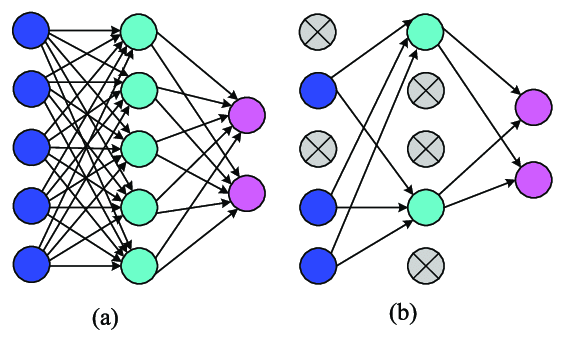
\includegraphics[width=10cm]{images/Dropout.png}
  \caption{ (a) Neural network (b) After applying dropout }
  \label{fig:Dropout}
\end{figure}

Dropout can be adjusted within different layers of a transformer model. Setting the dropout to a value between 0 and 1 expresses the probability of dropout being applied within specified layers. For example, setting the dropout probability to 0.1 implies that each neuron within a particular layer has a 10\% probability of being dropped out during training.

\cite{BERT-dropout} investigated the effect of changing dropout parameters for different layers of BERT for news classification. They compared using dropout on attention probabilities, fully connected layers and a combination of both, with dropout probabilities between 0.1 and 0.6. They discovered that using dropout on just the attention probabilities caused more overfitting, and just using dropout on hidden layers caused a degradation in performance. However, they did discover that regularising a BERT model using dropout on both fully connected layers and attention probabilities provided the most optimal results, particularly when they used a high value for attention probability (0.5) and a low value for hidden layer probability (0.2). This paper primarily investigated using dropout within the context of fine-tuning BERT but not feature extraction.

Within the context of biomedical relation extraction, publications tend to contain more complex information, making it easy for BERT to learn patterns that overfit the training data. Dropout could potentially be useful in this case since the network can be encouraged to identify trends that are more generalisable to other biomedical documents.

%==================================================================================================================================
\chapter{Research Questions}

\section{Introduction}
Performing research into existing relation extraction methods has revealed insightful information that can be translated into the domain of biomedical relation extraction. As such, several research questions can be proposed to investigate elements impacting the overall quality of model performance. These questions primarily focus on the impact of altering input text, as inspired by \cite{architectures} and \cite{mask}; however, there is also a proposal to investigate regularisation methods that can reduce the complexity of patterns learned by transformer models. The model primarily being focused on for this implementation is the BERT model, which is the state-of-the-art transformer model used for this task. 

\subsection{Will classifying entity representations be more effective than classifying [CLS] representations?}

One of the factors impacting model quality is selecting a suitable sentence representation from BERT's output. With several implementations of biomedical relation extraction, there is often a need for more exploration regarding the sentence representation being extracted. The most common choice is the [CLS] tag at the beginning of every sentence. \cite{architectures} suggests that more valuable information could be gained from extracting representations more specific to the entities of interest within the text. Their best results were obtained by adding unique tags at the beginning and end of entity mentions. Biomedical documents tend to contain large and convoluted entities that can be difficult for BERT's self-attention mechanism to interpret. Including tags that indicate the position of entities within text has been beneficial since they provide more information about where they are located within text. This research focuses on discovering whether using entity-specific representations from entity markers is more effective than regular [CLS] representations within the biomedical domain.  

\subsection{How much entity mention information does BERT require within the text input?}

Following the research performed by \cite{mask}, there is the possibility that altering how entities are represented in input text can have an impact on the quality of the model output. With a standard unmodified text input, BERT might learn the "wrong" information from input text. For example, it might just look at the entity names and recall a particular relation for the entities based on a previous sentence, making it more likely for the model to ignore the context surrounding the entities during training and creating a model over-fitting to the training data. This research question will investigate how much entity information is best to provide to BERT in order for the model to produce more optimal results, including providing both entity mentions and surrounding sentence context, providing just the entity types and the context, and just providing the context of the sentence whilst omitting all of the entity information. Both the [CLS] tags and the entity representation markers will be extracted and compared for these variations since they can elucidate the differences between these models. 

\newpage
\subsection{What is the effect of changing dropout levels for different sentence representations?}

Biomedical publications tend to be particularly structurally complex; Entities tend to be long-winded and be related to several instances mentioned within sentences. Consequently, there is a high possibility that transformer models will interpret noisy features from these inputs and derive very specific patterns that will not generalise well to the rest of the data. Introducing dropout to these models can encourage them to generalise; however, there is the risk of performance reduction if too many neurons are set to zero during training. As such, this research question investigates which probability balances generalisation and model performance on a system that includes both entity mentions and context. Specifically, there will be an investigation into how certain dropout levels affect the output quality for different sentence representations extracted from the input sentences.

\chapter{Methods}

\section{DrugProt}
The dataset being used to conduct these research questions is the DrugProt dataset, which was created by \cite{dataset} to promote the development and evaluation of systems that can automatically detect chemical-protein relations. This corpus contains thousands of PubMed abstracts manually annotated by domain experts, who labelled all mentions of chemicals and genes and all binary relationships between them corresponding to relevant relation types. This makes the annotations high-quality and based on experimental evidence. DrugProt is one of the most extensive protein-drug interaction datasets, with over 18000 unique targets and 38000 interactions. This dataset would be helpful for biomedical relation extraction since it contains a large amount of information about chemicals and genes that models can learn from and use within their predictions.

%The DrugProt overview paper written by \cite{overview} summarises previous submissions to the DrugProt track, comparing different results obtained and elaborating on methods that were undertaken. This overview paper provides valuable insight into modern methodologies for biomedical relation extraction. For example, 30 out of 32 submissions involved the use of transformer language models, emphasising that they are the current state-of-the-art method within this domain. This is useful knowledge for performing research on further modifications that can be made to these transformer models in order to improve their performance.  As observed within the overview paper written by \cite{overview}, there are several gaps that can be expanded upon through further research. As such, a number of research questions can be proposed in order to provide further insight into how to obtain better performance using transformer models.

\subsection{Training and Development Sets}
There are 13 different relations within this dataset, with their mentions varying in quantity across the training and development sets. These represent relations between chemicals and genes, covering most of the essential relations from biochemical, pharmacological, and biomedical perspectives. 

\begin{figure}[h]
\begin{center}
\begin{tabular}{||c c c||} 
 \hline
 Classes & Training & Test\\ [0.5ex] 
 \hline\hline
 INDIRECT-DOWNREGULATOR & 1330 & 332 \\ 
 \hline
 INDIRECT-UPREGULATOR & 1379 & 302\\
 \hline
 DIRECT-REGULATOR & 2250 & 458\\ 
 \hline
 ACTIVATOR & 1429 & 246\\
 \hline
 INHIBITOR & 5392 & 1152\\ 
 \hline
 AGONIST & 648 & 131\\
 \hline
 ANTAGONIST & 968 & 218\\ 
 \hline
 AGONIST-ACTIVATOR & 29 & 10\\
 \hline
 AGONIST-INHIBITOR & 13 & 2\\ 
 \hline
 PRODUCT-OF & 921 & 158\\
 \hline
 SUBSTRATE & 2003 & 495\\ 
 \hline
 SUBSTRATE\_PRODUCT-OF & 25 & 3 \\
 \hline
 PART-OF & 886 & 258\\ 
 \hline
\end{tabular}
\caption{A table specifying the number of each relation that occurs within the relevant dataset.}
\end{center}
\end{figure}
\newpage
\subsection{Document Structure}

There are 3499 documents within the training set and 750 documents within the test set. Each document has the following structure:
\begin{itemize}
    \item \textbf{PubMedID}: The ID of the relevant PubMed article.
    \item \textbf{Article Title and Abstract}: The text from which relations will be extracted.
    \item \textbf{Entities}: A nested dictionary of chemicals and genes found within the text.
    \item \textbf{Relations}: A list of relations between a subset of entities discovered in the text.
\end{itemize}

Each document only contains the title and abstracts since they are usually the most informative parts of scientific articles, providing a concise summary of the research presented in the full text. Each entity within a document has the following structure:
\begin{itemize}
    \item \textbf{Type:} This specifies whether the entity is a gene or a chemical
    \item \textbf{Start:} The index where the entity appears within the text
    \item \textbf{End:} The index where the entity finishes within the text
    \item \textbf{Entity Name:} The name of the chemical or gene that appears in the text
\end{itemize}

Unlike several other datasets, the DrugProt dataset specifies the indices of where a specific entity mention occurs within text, which is particularly useful for finding and classifying specific relations. This elucidates which part of the sentence a particular relation is specified and prevents any confusion caused by manually interpreting and labelling sentences as having a particular relation. Each relation has the following structure:
\begin{itemize}
    \item \textbf{Type:} This specifies the type of relation shared between the two entities, e.g. INHIBITOR
    \item \textbf{Arg1:} The key of a particular chemical entity involved in a relation
    \item \textbf{Arg2:} The key of a particular gene entity involved in a relation
\end{itemize}

This can be used when highlighting particular entities of interest within the sentence, as they can be verified against the list of relations for their relevant document.

\section{PubMedBERT}
The transformer model being used in this implementation is PubMedBERT. This is because, as seen from \cite{PubMedBERT}, PubMedBERT tends to ensure that particular entities remain intact post-tokenisation, which can help improve the model's interpretation of the text. The PubMedBERT and tokeniser being used will be pre-trained on abstracts and full text of biomedical documents to increase the frequency of particular biomedical terms being observed by BERT a priori. Various custom tags required to investigate the established research questions, namely "[E1]", "[/E1]", etc., were then added to the token's vocabulary in order to prevent them from being split up by the tokeniser. For example, if '[E1]' is not added to the model's vocabulary, it would be tokenised as '[','e1',']' and could be misinterpreted during training.

\section{Data Pre-Processing}

It was verified by \cite{tag} that less than 1\% of the total annotations recorded within the training set occur across sentences. Consequently, this implementation primarily focuses on relations that occur within a single sentence. This reduces the complexity of the implementation since it does not need to consider seemingly arbitrary occurrences of cross-sentence relations. The indices of each annotated entity being specified are helpful in this case since it simplifies the process of identifying which entities occur in particular sentences.

Segtok is a segmentation library that was used to split the sentences within the documents. Their \emph{split\_single()} function provides a more sophisticated approach to splitting sentences than merely using python's split function since it takes complex grammatical structures of sentences into account. This is particularly important within biomedical text, where there is a high occurrence of abbreviations and figures whose structure needs to be retained to be correctly interpreted.

One of the issues experienced with the DrugProt dataset was that some entities weren't indexed correctly. For example, the index of a particular mention might cross over into an adjacent term within the sentence or, in some cases, cross sentence boundaries. Only a small number of entities crossed these sentence boundaries, so they were removed from the dataset.

\subsection{Will classifying entity representations be more effective than classifying [CLS] representations?}

In order to investigate this question in a controlled manner, there must be consistency regarding the textual input that the representations will be taken from. If the sentences were structurally different, the results likely would not reflect the true nature of using different representations. Figure \ref{fig:Sentence} is an example sentence from the DrugProt dataset that will be used to demonstrate the different alterations that will be made to the input text.

\begin{figure}[h]
    \centering
    \fbox{\begin{minipage}{30em}
\centering
EACA inhibited the binding of plasmin to gp330 slightly more than the binding of plasminogen to gp330.
\end{minipage}}
  \caption{Example sentence from the DrugProt dataset. It consists of a chemical, namely EACA, and three genes, namely plasmin, plasminogen and gp330. }
  \label{fig:Sentence}
\end{figure}For this research question, special tags will be added to the text to highlight entities of interest to BERT during training. These tags will be:

\begin{itemize}
\item $\textbf{[E1]/[/E1]}$ for annotated chemicals
\item $\textbf{[E2]/[/E2]}$for annotated genes
\end{itemize}

This is demonstrated in figure \ref{fig:Tagging}, which depicts a sample sentence from one of the documents within the DrugProt dataset as mentioned in figure \ref{fig:Sentence}. In this case, EACA is a chemical and is therefore encased in $[E1]/[/E1]$ tags, whilst plasmin is a gene, and is therefore encased in $[E2]/[/E2]$ tags. These sentences will then be tokenized, and the [CLS] and [SEP] tags will be added to the beginning and the end of each sentence, respectively. 

\begin{figure}[h]
    \centering
    \fbox{\begin{minipage}{30em}
\centering
[E1] EACA [/E1] inhibited the binding of [E2] plasmin [/E2] to gp330 slightly more than the binding of plasminogen to gp330.
\end{minipage}}
  \caption{Example sentence with entity marking tagging scheme.}
  \label{fig:Tagging}
\end{figure}

In the case of using the [CLS] representation for classification, each entity is labelled with markers; however, only the embedding for the [CLS] tag is taken for each sentence. The embedding representation of the [CLS] tag will always be at the zeroth index of the resultant list of embeddings and is, therefore, trivial to obtain. In this case, the embedding size will be 768 since this is the size of the embedding vectors within BERT. This is reflected in figure \ref{fig:EMCLS}.

In the case of using entity representations, the entities are labelled with markers, and the start tags for each entity are extracted and concatenated. The indexes at which these embeddings occur will be found by finding the indexes at which the entity start tokens appear within the tokenised text. Since the embeddings are being concatenated, the length of the resultant vectors will be $2*768 = 1536$. This is reflected in figure \ref{fig:EMES}.

\subsection{How much entity mention information does BERT require within the text input?}

For this research question, one representation to test would be to remove all information about the entity mention, which could be achieved by using the generic built-in [MASK] tag that BERT uses for pre-training. The idea is that it is a mechanism that BERT is already familiar with, and it does not provide any additional information about the entity. The results using this entity masking technique would provide information about how much context outside of entity mentions the model relies on in order to create accurate relation predictions. Using the same sample sentence from figure \ref{fig:Sentence}, replacing entity mentions with [MASK] tags can be demonstrated in figure \ref{fig:Mask}.

\begin{figure}[h]
    \centering
    \fbox{\begin{minipage}{30em}
\centering
[MASK] inhibited the binding of [MASK] to gp330 slightly more than the binding of plasminogen to gp330.
\end{minipage}}
  \caption{Example sentence with general masking employed}
  \label{fig:Mask}
\end{figure}

In a similar fashion to the previous research question, we can examine the effect of altering the input text on the sentence representations extracted from the sentence. Changing the input text can have an impact on both the [CLS] representation of the sentence, in addition to the new [MASK] entity representations within the text. This method will be referred to as the \textbf{General Masking} method. Figure \ref{fig:EMMASK} illustrates extracting the [CLS] representation from the sentence.

\begin{figure}[htb]
    \centering
    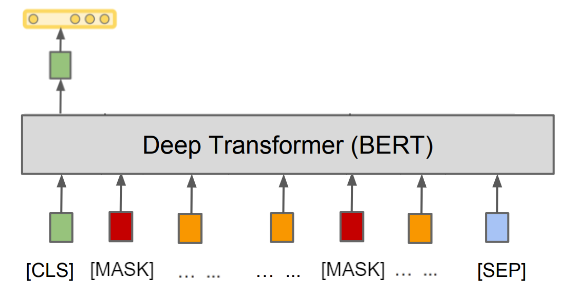
\includegraphics[width=10cm]{images/CLSMASK.png}
  \caption{Entity Representation Diagram}
  \label{fig:EMMASK}
\end{figure}

Within the previous research question, the entity representation was extracted from each of the tags at the start of the entity mentions. In this case, these tags will not be present, therefore the entity representation will be extracted from the entity masks. As before, these representations will then be concatenated together, forming vectors of size 1536. This is represented in figure \ref{fig:Masked}. During concatenation, the [MASK] representation of the chemical within the sentence will always be before the [MASK] representation of the gene to ensure consistency regarding the structure of the resultant vectors.

\begin{figure}[htb]
    \centering
    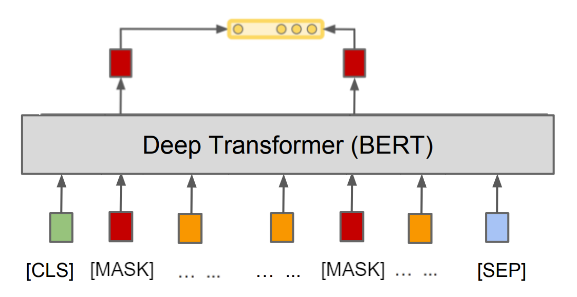
\includegraphics[width=10cm]{images/EMMask.png}
  \caption{Extracting Mask representations}
  \label{fig:Masked}
\end{figure}

Another representation to test would be the removal of entity mentions as before, but providing some indicator of the type of entity being represented. This could be achieved by creating special tokens [CHEM] and [GENE] to indicate the type of entity being masked. Using these tags can provide BERT with more information regarding the role of the masked entity within the sentence, in addition to its position within the sentence. This entity mask representation is expressed using the example sentence in figure \ref{fig:Special}.

\begin{figure}[h]
    \centering
    \fbox{\begin{minipage}{30em}
\centering
[CHEM] inhibited the binding of [GENE] to gp330 slightly more than the binding of plasminogen to gp330.
\end{minipage}}
  \caption{Example sentence with special masking employed}
  \label{fig:Special}
\end{figure}

\newpage
The [CLS] and entity representations for this \textbf{'Special Masking'} method will be taken in the same way as demonstrated for the general masking method, but with [CHEM] and [GENE] tags instead of [MASK] tags. The entity representation of this variation can be demonstrated in figure \ref{fig:EMCHEM}. An investigation into the effectiveness of providing both the entity and the mention will come from the results obtained from the previous research question. If there is very little difference in the classification results for each architecture, then it implies that BERT relies entirely on the context surrounding the entities in order to determine the classification of the sentence.

%\begin{figure}[htb]
%    \centering
%    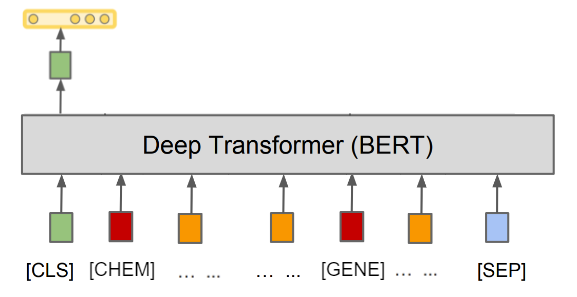
\includegraphics[width=10cm]{images/CLSCHEM.png}
%  \caption{Entity Representation Diagram}
%  \label{fig:EMCHEM}
%\end{figure}

\begin{figure}[htb]
    \centering
    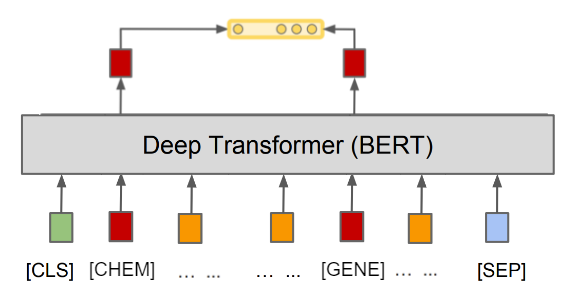
\includegraphics[width=10cm]{images/Chem.png}
  \caption{Entity Representation Diagram}
  \label{fig:EMCHEM}
\end{figure}

\subsection{What is the effect of changing dropout levels for different sentence representations?}

BERT has two parameters: \textbf{attention\_probs\_dropout\_prob} which applies dropout to BERT's attention layers and \textbf{hidden\_dropout\_prob}, which applies to all of BERT's feed-forward intermediate layers. Figure \ref{fig:Drop} shows an example of one of BERT's layers, where the attention dropout within the self-attention block is equivalent to \textbf{attention\_probs\_dropout\_prob}, whilst the hidden dropout is equivalent to the \textbf{hidden\_dropout\_prob}. 

BERT's attention layers are responsible for computing the contextualized representations of each token in the input sequence. It is possible that BERT's self-attention can introduce noise when determining the importance of particular entities within a sentence, therefore increasing dropout for these layers could reduce the effect of the noise within the model. However, it is possible that too much dropout could remove too much information about entity importance, and begin to decrease performance. 

The hidden layers are responsible for transforming representations into higher-level features that can be used for text classification. Increasing the dropout for the hidden layers could have the effect of smoothing the output of the GELU activation function by reducing the impact of individual neurons. Similarly for these layers, an increase of dropout can have a detrimental effect on the output for each layer.

\begin{figure}[htb]
    \centering
    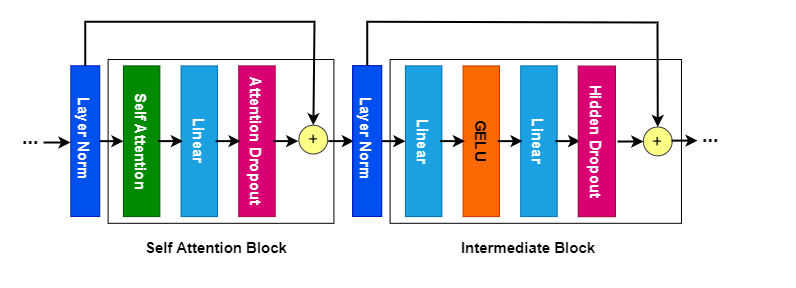
\includegraphics[width=16cm]{images/Drop.png}
  \caption{Example of the structure of one of BERT's 12 layers. It consist of a self-attention block and an intermediate block}
  \label{fig:Drop}
\end{figure}

Within their paper, \cite{BERT-dropout} restricted the dropout levels to be between 0.1 and 0.6, stating that anything larger than 0.6 resulted in a degradation in performance. Since feature extraction will be used within this implementation instead of fine-tuning, there is a possibility that the results for changing the dropout parameters will differ compared to the optimal parameters obtained within their results. The model will be tested by increasing dropout values in increments of 0.1 uniformly across each parameter to see the effect on the predictions of the overall model. The final parameter to be tested will be 0.7 to see if the performance degradation exists at this level within the implementation. It is possible that the level of dropout required for regularisation is dependent on the type of sentence representation used, therefore these values will be tested on both [CLS] and entity representations from sentences contain both context and mention.

\subsection{Relation Statements}
To train the model there needs to be a fair number of positive and negative potential relations. This is so that BERT can learn enough enough negative examples to encourage it to detect more accurate patterns indicating relations. If there aren't any negative examples included there is a chance that the model will assume that there will always be a relation between a chemical and a gene if they happen to occur within the same sentence. In a single sentence, there are potentially several relations between chemicals and genes. One way of gaining enough samples is to take the Cartesian product of all of the chemicals and all of the genes in one sentence, as demonstrated with figure \ref{fig:Sentence}:

\begin{figure}[htb]
    \centering
    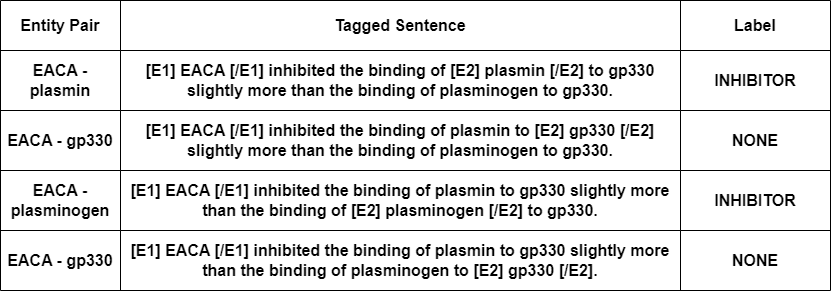
\includegraphics[width=14cm]{images/Tags.png}
  \caption{Example of using cartesian product to produce entity pairs and tag them within the sentence}
  \label{fig:Tags}
\end{figure}

\section{Logistic Regression}
 The choice of model used in conjunction with BERT's input can have a significant impact on the quality of the overall output. Logistic regression appears to be the most suitable classification model to use for this task, since it can be used to model the relationship between the extracted features and the target variable. This allows for easy interpretation of the importance of each feature for text classification. It is usually used for binary classification, however it can be extended to accommodate multi-class, meaning it can classify sentence representations into each relation category. It can also handle high-dimensional data, such as the 768-sized vectors outputted by BERT. For feature extraction, the embeddings from PubMedBERT will be fed into Scikit learn's LogisticRegression model with the following parameters:

\begin{itemize}
    \item \textbf{class\_weight} = 'balanced'
    \item \textbf{solver} = 'saga'
\end{itemize}

Since the majority of combined chemicals and genes won't form a relation, it is possible that the classifier won't take the minority cases into account and as a blanket statement predict every possible relation as having no relation. In order to mitigate this class imbalance, setting class weight to 'balanced' ensures that minority classes are given the same weight as majority classes when predicting relations. Since there is a large amount of data being used within the model, solver was set to 'saga' to perform faster computations.

% \section{Implementation Issues}

%\subsection{Dataset Issues}
%There are several features of the dataset that caused some time-consuming issues.

%\begin{itemize}
%    \item \textbf{Index annotation issues:} One of the primary issues involved a lack of thorough testing of the dataset, creating a myriad of time-consuming issues. For example, some of the indexes for annotations were inaccurate and included some other aspects of the adjacent words for some sentences. Some of the entity names had a '.', meaning that segtok was assuming that it was part of a sentence and splitting it up. This lead to several disjointed tags blah blah 
%    \item \textbf{Entity annotation issues:} Upon closer inspection of the annotations, it was discovered
%\end{itemize}

%Talk about the '.' in some entity names, how some were across sentences etc.

%\subsection{Entity Tag Issues}
%Talk about how you had to add the tags as new tokens to be interpreted by the transformer.
%The lack of spacing around tags, causing them to not be picked up by the tokenizer.
%Segtok issues

%==================================================================================================================================
\chapter{Evaluation} 
%How good is your solution? How well did you solve the general problem, and what evidence do you have to support that?
%Ask specific questions that address the general problem.
%Answer them with precise evidence (graphs, numbers, statistical analysis, qualitative analysis).
%Be fair and be scientific.
%The key thing is to show that you know how to evaluate your work, not that your work is the most amazing product ever.

%Superior architecture?

\section{Evaluation Metrics}
Suitable evaluation metrics needed to be established in order to sufficiently compare the differences between architectures and regularisation methods. This involves comparing the true positive (TP), true negative (TN), false positive (FP) and false negative (FN) values for each class. In this case, the following metrics were used:

\begin{itemize}
    \item \textbf{Precision:} This determines how many of the correctly predicted classes are positive. It is equivalent to the ratio of true positives to the sum of true positives and false positives.
    \begin{equation}
    Precision = \frac{TP}{(TP + FP)}
    \end{equation}
    \item \textbf{Recall:} This determines the number of positive classes that were correctly predicted. It is equivalent to the ratio of true positives to the sum of true positives and false positives. 
    \begin{equation}
    Recall = \frac{TP}{(TP + FN)}
    \end{equation}
    \item \textbf{F1-Score:} This is equivalent to the harmonic mean of precision and recall, and is generally considered the most important metric, as it can reflect issues with class imbalance within the dataset.
    \begin{equation}
    F1-Score = 2 x \frac{(Precision*Recall)}{(Precision + Recall))}
    \end{equation}
    \item \textbf{Confusion Matrix:} A table that describes the performance of a classification model where the true values of the test set are known. The desire is for the main diagonal of the table to contain the largest number.
\end{itemize}

\section{Will classifying entity representations be more effective than classifying [CLS] representations?}

\subsection{Results}
\begin{figure}[h]
\begin{center}
\begin{tabular}{||c c c c||} 
 \hline
 Embeddings & F1-Score & Precision & Recall \\ [0.5ex] 
 \hline\hline
 [CLS] & 0.39 & 0.74 & 0.35 \\ 
 \hline
 [E1]/[E2] & \textbf{0.61} & \textbf{0.81} & \textbf{0.56}\\
 \hline
\end{tabular}
\end{center}
\caption{Evaluation Metrics for [CLS] representations and Entity representations}
\label{fig:qn1}
\end{figure}

When comparing sentence representations, there was a significant increase in performance for classification using entity start ([E1]/[E2]) tags compared to [CLS] tags, with approximately 20\% difference in F1-Score between them. This can be observed in figure \ref{fig:qn1}, which also presents the precision and recall for each input type. Entity representations appear to exhibit a larger precision value, which implies that they have more success with positively identifying relations within each class. They also provide a significantly larger recall value, implying that they are able to detect more general patterns for each class, resulting in better predictions. It is worth noting that there is a large difference in precision and recall values for both representations, which indicates that there is a potential issue of class imbalance for both models. More information about how sentences have been classified can be obtained by finding the confusion matrices for each representation type.

\begin{figure}[htb]
    \centering
    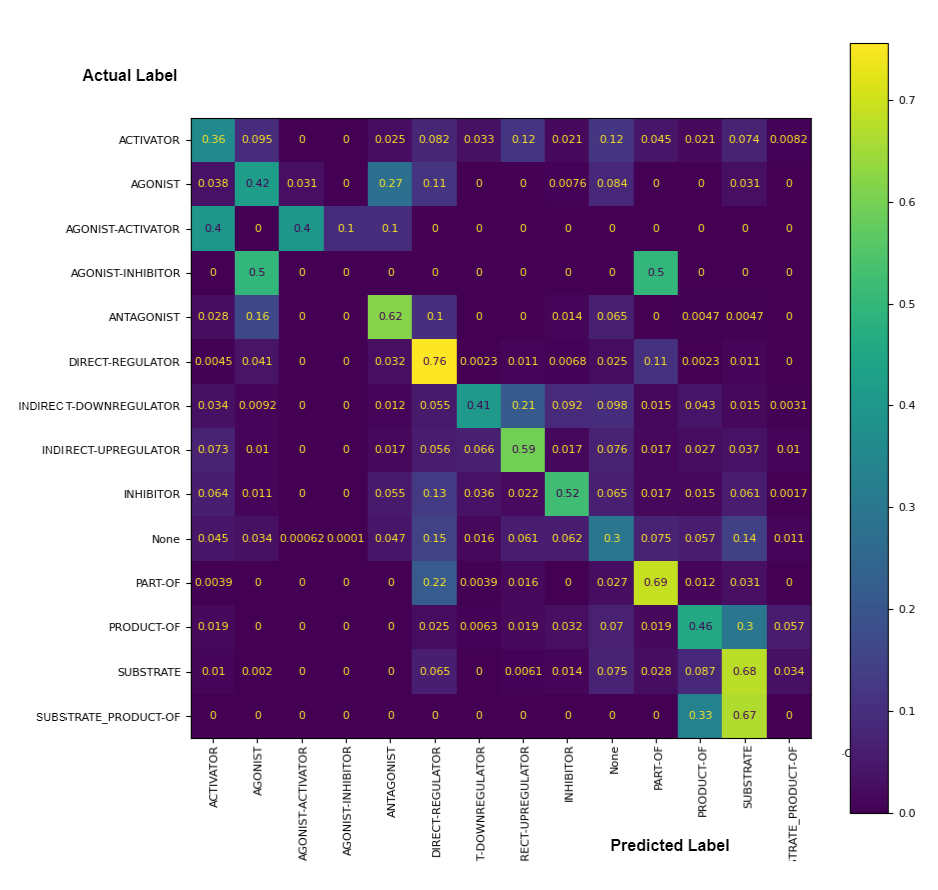
\includegraphics[width=16cm]{images/cls_mult.png}
  \caption{Confusion matrix representing the accuracy of classifications for [CLS] representation}
  \label{fig:cls_mat}
\end{figure}

The confusion matrix for [CLS] representations is presented in figure \ref{fig:cls_mat}. It can be observed that some of the larger percentages for each entry aren't focused on the main diagonal. Particular anomalies can be found for the AGONIST-INHIBITOR and SUBSTRATE-PRODUCT-OF relations, where none of the sentences relating to these classes were classified correctly. This is likely due to the severe lack of instances for these relations within both the training and test sets. Consequently, there wasn't enough data provided to the model in order to it to recognise particular patterns for these relations, making it more likely for those sentences to be predicted as different classes. Interestingly, both of these relations were predicted into classes that were thematically similar. For example, SUBSTRATE-PRODUCT-OF sentences were either predicted as belonging to the classes SUBSTRATE and PRODUCT-OF. It is possible that these phrases are common within these classes, and that is what the model has learned from.

It can be observed that there are a particularly large number of non-zero entries for the 'None' and 'DIRECT-REGULATOR' classes. This is likely an issue of class imbalance, since these entries contained the most instances within the training set. This explains the low recall values demonstrated in figure \ref{fig:qn1}, since the model has likely learned from these large instances the most during training and has not picked up on the nuances of less frequent patterns. Consequently sentences are most likely to be classified as one of these classes.

\begin{figure}[htb]
    \centering
    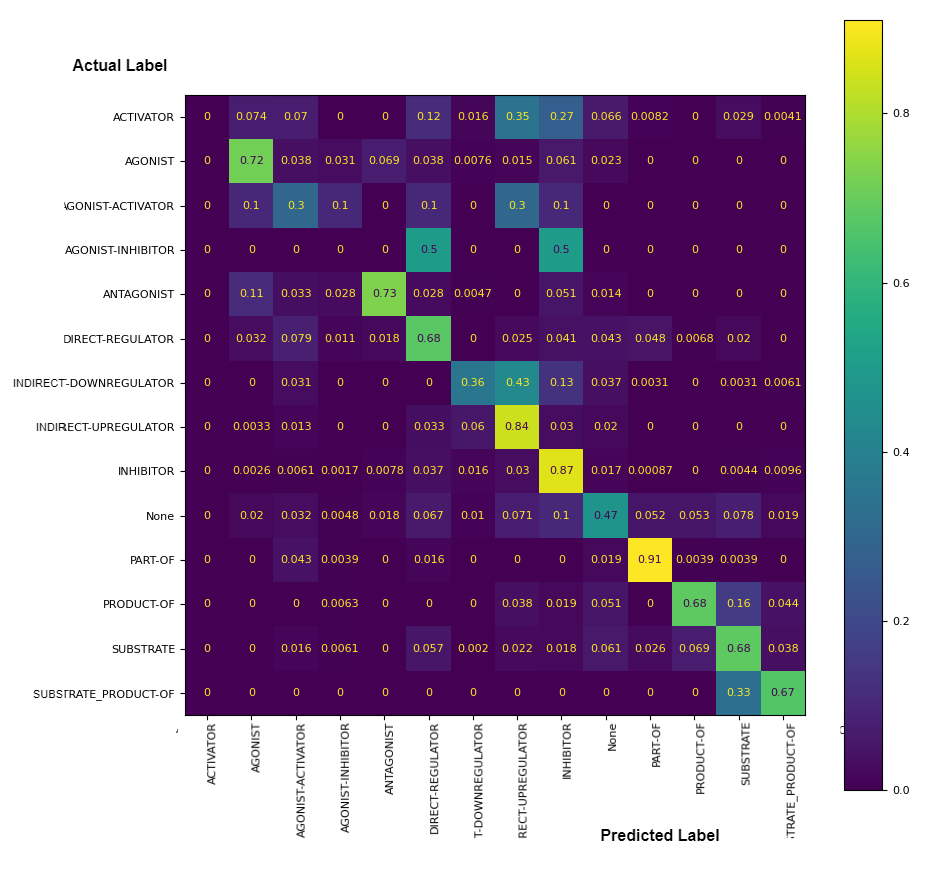
\includegraphics[width=16cm]{images/ent_mult.png}
  \caption{Confusion matrix representing the accuracy of classifications for entity representation}
  \label{fig:ent_mat}
\end{figure}

\newpage
The confusion matrix for entity representations is presented in figure \ref{fig:ent_mat}. It can be observed that a higher percentage of sentences within each category are correctly classified, and that there are fewer large percentage values falling outside of the main diagonal. This model correctly identified the majority of sentences for SUBSTRATE-PRODUCT-OF, however it appears to have incorrectly identified all of the ACTIVATOR sentences. It is possible that providing entity representations has made the model overfit to phrases adjacent to the mentions, making BERT's self-attention mechanism provide them with a higher weight than necessary during training.

Despite the class imbalance, using entity representations almost doubled the performance of the model, which demonstrates that using this representation provides significantly more information about how entities are related to one another compared to [CLS] representations. It is likely that the increased dimensionality provided by concatenating both chemical and gene representations is the primary cause for this performance improvement. As the dimensionality of the input space increases, the number of possible decision boundaries that can separate the data points also increases, therefore there are more degrees of freedom to separate each class. This increased separation means that there is less confusion with which class any particular sentence should be classified as.

\section{How much does BERT rely on entity mention information within the text input?}

\subsection{Results}

Figure \ref{fig:F1} compares the F1-Scores obtained from using entity markers versus using both general ([MASK]) and special ([CHEM]/[GENE]) masks. It can be observed that extracting a sentence entity representation from the special masks provides the best F1-score, followed by general masking, and then entity marking.  

\begin{figure}[htb]
    \centering
    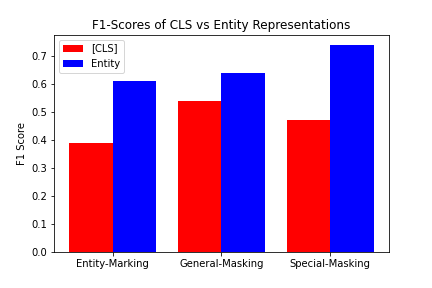
\includegraphics[width=12cm]{images/F1.png}
  \caption{Table comparing the F1-Scores between [CLS] and entity representations for entity marking and entity masking methods}
  \label{fig:F1}
\end{figure}

\newpage
In general, there is a clear distinction between the F1-Scores gained by using the [CLS] representation compared to using the entity representation, further solidifying the fact that using entity representations provides a significant edge to the quality of classification results. However, there is a difference in the effectiveness of the types of masking used, depending on the type of sentence representation being used for BERT's output. Both representations experience a general improvement of metrics, however [CLS] embeddings seem to benefit more from using general masking, whilst entity tag representations benefit more from special masking. It is possible that [CLS] representations perform better when using [MASK] tags because these are used for the task of MLM during pre-training. This involves attempting to guess missing words in sentences, with the missing word being shrouded by the [MASK] tags. Including these tags during training make it easier for BERT to recognise the task, and therefore the [CLS] tags are able to prioritise information involving the surrounding context of the entities.

Representing context and entity type provided the best F1-score, with a general improvement of entity representation results of around 10\%. This is likely due to the reduction in input complexity. Chemical and gene names have the propensity to be extremely complicated and long-winded, and can produce a large number of tokens when tokenised. If both context and mention are included within the input, this can have a negative impact on BERT's self-attention mechanism, since it may lose the ability to capture the entire entity as a single unit and therefore lose important information, regardless of whether or not positional entities are included. 

The mechanism may also assign disproportionately high weights to these entities as they contain more tokens compared to other parts of the sequence, which can over-emphasise these names at the expense of other semantic information within the sequence. This can reduce the efficiency of the model in capturing relationships within different parts of the input sequence, therefore reducing the effectiveness of the overall model. Omitting entity mentions may have been more beneficial in this case, since it simplifies the input sequence and allows BERT to capture more of the semantics of the sentence outside of the entity mentions. Figure \ref{fig:Long} is an example of one of the many chemicals annotated within the DrugProt corpus, and demonstrates the number of tokens that could potentially be obtained from one entry. 

\begin{figure}[h]
    \centering
    \fbox{\begin{minipage}{30em}
\centering
 R-(+)-[2,3-dihydro-5-methyl-3-[(morpholinyl)methyl]pyrrolo[1,2,3-de]-1,4-benzoxazinyl]-(1-naphthalenyl)methanone mesylate
\end{minipage}}
  \caption{Example chemical name. This produces 60 tokens when tokenised.}
  \label{fig:Long}
\end{figure}


%\subsection{Binary Classification}

%We can also compare the performance of binary classification, where the model determines if a particular sentence contains a relation or not, regardless of what the relation is. It is worth observing the fact that the binary classification results for [CLS] embeddings and whatever fixed-length representation it is being compared against (Markers or masks) remains constant regardless of the architecture used. The results of binary classification express around a 10\% improvement across all metrics for classifying alternate tags compared to [CLS] tags.
% Explain why this might be
% Maybe refer specifically to logistic regression and how it's set up
% Could maybe write a section dedicated to changing logistic regression depending on what is being tested
% Might change this depending on the results

%\begin{figure}[h]
%\begin{center}
%\begin{tabular}{||c c c c||} 
% \hline
% Architecture & F1-Score & Precision & Recall \\ [0.5ex] 
% \hline\hline
% [CLS] & 0.70 & 0.75 & 0.69 \\ 
% \hline
% Entity & \textbf{0.79} & \textbf{0.82} & \textbf{0.78}\\
% \hline
%\end{tabular}
%\end{center}
%\caption{Binary classification for Feature Extraction}
%\end{figure}

\section{What is the effect of changing dropout levels for different sentence representations?}

\subsection{Results}
If Dropout does indeed provide a more generalisable outcome, then this should be observed within the evaluation metrics of the training and test sets. The assumption is that with low amounts of dropout, there should be a higher difference between the F1-scores of the training set compared to the test set. As more dropout is applied, this difference should theoretically decrease due to an increase in generality. Figure \ref{fig:F1} shows the results of introducing different levels of dropout on entity representations.

\begin{figure}[htb]
    \centering
    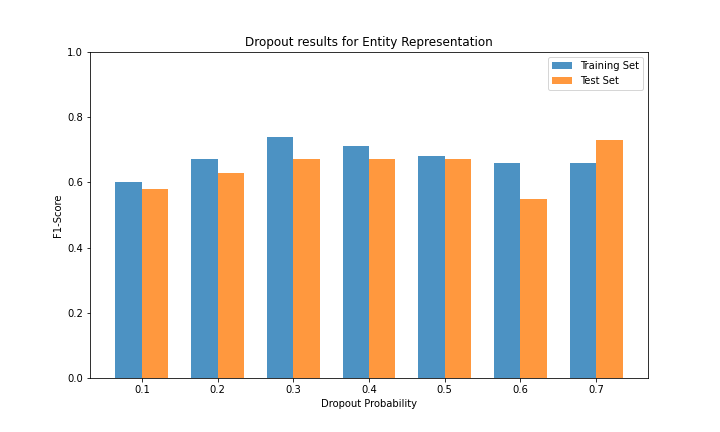
\includegraphics[width=14cm]{images/EntityDrop.png}
  \caption{Table comparing the F1-Scores between training and test sets across different levels of dropout for entity representations}
  \label{fig:F1}
\end{figure}

\newpage

The entity representation results appear to adhere to this assumption until the highest dropout probabilities are applied to the model. The training set performance appears to increase in F1 score until it reaches a maximum at value 0.3, where it gradually decreases and levels off for higher probabilities. It is possible that enough neurons were set to 0 in this example to remove some of the noise introduced during training, however not enough that the model is able to discern a concrete pattern to apply to the test set. The test set performance also appears to improve as the dropout levels increase, until it reaches dropout level 0.6, where it appears to destabilise. For dropout probability 0.7, there appears to be an anomalous result, since the test set appears to have performed better than the training set. It is possible that in this case, the patterns were obscured so much by dropout that the model learned incorrect trends that happened to align with the test set more than the training set.

The smallest difference between the training and test sets can be observed at value 0.5, implying that this is the optimal probability for encouraging generality within the model. There is approximately a 10\% increase in F1-score for both training and test sets when compared to the results with minimal dropout. 

It can be observed within figure \ref{fig:F1cls} that there is more of a trend of over-fitting when it comes to [CLS] representations with minimal dropout when compared to entity representations. In this case, dropout does provide a significant improvement for generalisation as the dropout probability is increased. The training set displays a similar trend to the training set for entity representations, where the F1 score increases to a maximum at 0.3, and decreases thereafter. However, in this case once dropout reaches a minimum F1 score 0.5, the training set begins to increase again, where it reaches a maximum at 0.7. 

The difference between the training and test sets are minimised at dropout level 0.6, where the training F1 score experiences no improvement, whilst the test set F1 score improves by around 10\%. Since the [CLS] tokens represent the entire sentence, the attention layer may be more likely to introduce noise as it attempts to set weights for the whole sequence. Increasing dropout may reduce this noise, and learn more appropriate patterns within the data.

\begin{figure}[htb]
    \centering
    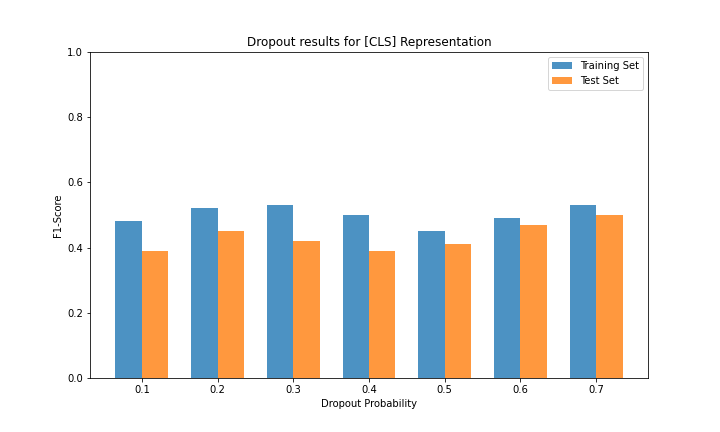
\includegraphics[width=14cm]{images/CLSDrop.png}
  \caption{Table comparing the F1-Scores between training and test sets across different levels of dropout for [CLS] representations}
  \label{fig:F1cls}
\end{figure}

It is worth noting that there was there was a fair amount of variance experienced when running the data, and it is possible that the results would differ slightly when reproducing the data. Since the output for BERT remained consistent throughout each run, the common denominator was the logistic regression model. This is likely because the model can converge to a different set of coefficients during optimization, and change the class bounds within the model.

%\begin{figure}[h]
%\begin{center}
%\begin{tabular}{||c c c c c||} 
% \hline
% Embeddings & Dropout & F1-Score & Precision & Recall \\ [0.5ex] 
% \hline\hline
% [CLS] & 0.1 & 0.39 & 0.74 & 0.35\\ 
% \hline
 %Entity-Start & 0.1 & 0.61 & 0.81 & 0.56\\
 %\hline
 %[CLS] & 0.2 & 0.45 & 0.74 & 0.39\\ 
 %\hline
 %Entity-Start & 0.2 & 0.63 & 0.80 & 0.59\\
 %hline
 % [CLS] & 0.3 & 0.42 & 0.75 & 0.36\\ 
% \hline
% Entity-Start & 0.3 & 0.67 & 0.79 & 0.63\\
% \hline
% [CLS] & 0.4 & 0.39 & 0.74 & 0.35\\ 
% \hline
% Entity-Start & 0.4 & 0.67 & 0.80 & 0.63\\
% \hline
 %[CLS] & 0.5 & 0.05 & 0.06 & 0.12\\ 
 %\hline
 %Entity-Start & 0.5 & 0.58 & 0.74 & 0.54\\ 
 %\hline
 %[CLS] & 0.7 & 0.44 & 0.74 & 0.39\\
 %\hline
 %Entity-Start & 0.7 & 0.73 & 0.77 & 0.72\\
 %\hline
%\end{tabular}
%\end{center}
%\caption{Dropout results for Entity Marker variation on the test set}
%\end{figure}

%\begin{figure}[h]
%\begin{center}
%\begin{tabular}{||c c c c c||} 
% \hline
% Embeddings & Dropout & F1-Score & Precision & Recall \\ [0.5ex] 
% \hline\hline
% [CLS]& 0.1 & 0.48 & 0.75 & 0.43\\ 
% \hline
% Entity-Start & 0.1 & 0.67 & 0.83 & 0.63\\
% \hline
% [CLS] & 0.2 & 0.52 & 0.73 & 0.46\\ 
% \hline
% Entity-Start & 0.2 & 0.67 & 0.84 & 0.63\\
% \hline
% [CLS] & 0.3 & 0.53 & 0.77 & 0.47\\ 
% \hline
% Entity-Start & 0.3 & 0.74 & 0.82 & 0.71\\
% \hline
% [CLS] & 0.4 & 0.50 & 0.78 & 0.44\\ 
% \hline
% Entity-Start & 0.4 & 0.71 & 0.83 & 0.68\\
% \hline
% [CLS] & 0.5 & 0.53 & 0.78 & 0.49\\
% \hline
% Entity-Start & 0.5 & 0.60 & 0.83 & 0.54\\ 
% \hline
% [CLS] & 0.7 & 0.56 & 0.77 & 0.51\\
% \hline
% Entity-Start & 0.7 & 0.66 & 0.81 & 0.62\\
% \hline
%\end{tabular}
%\end{center}
%\caption{Dropout results for Entity Marker variation on the training set}
%\end{figure}

%Increasing dropout levels appears to have the effect of increasing recall and F1-score for Entity start embeddings, therefore increasing the overall performance of the model. In this case, entity markers are more tailored to specific named entities within the text, therefore applying dropout can prevent overfitting to these specific entities and force the model to learn more robust features of the model.


%\begin{figure}[htb]
%    \centering
%    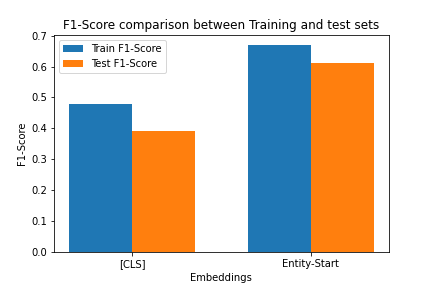
\includegraphics[width=14cm]{images/trainvtest.png}
%  \caption{Table comparing the F1-Scores between [CLS] and entity representations for entity marking and entity masking methods}
%  \label{fig:F1}
%\end{figure}

% Test dropout on entity masks

%In contrast, increasing dropout results in decreasing recall and F1-score for [CLS] embeddings, whilst precision remains relatively consistent. Recall determines the proportion of positive relations that were correctly identified. Increasing dropout may cause a degradation in performance in this particular context, since [CLS] embeddings represent an entire input sequence, and therefore applying dropout may introduce noise and therefore prevent the model from capturing the full context of the sentence.



% Explain why it might be good for entity start stuff

% Write up the rest of it
 
%==================================================================================================================================
\chapter{Discussion} 
It is entirely possible that using the logistic regression model in its current form reduces its ability to perform well when classifying the data. Since the input data is complex, it is important to tune the model so that it can accommodate the nuances of each class, and create more distinct hyperplanes so that each class can be correctly identified. There are several parameters for logistic regression that can be adjusted in order to improve model performance:

\begin{itemize}
    \item \textbf{C}: This represents the regularisation strength, which controls the weight the model puts on reducing the training error compared to reducing the complexity of the model. If this value increases, then the model will be less regularised, whilst a lower value results in a more regularised model.
    \item \textbf{Penalty}: This specifies an additional regularisation type that can be used on the model, either L1 or L2 regularisation. L1 reduces some coefficients to zero, which is typically useful for feature selection, any variables associated with coefficients that go to zero can be dropped. L2 reduces the size of all coefficients, which is useful if there are codependent features within the model.
    \item \textbf{Solver}: This represents the algorithm that is used to optimise the objective function used for logistic regression. Some are better at handling large datasets than others, and each one has a different level of support for different penalty functions. For example, the 'liblinear' solver is typically best for small datasets and can support both L1 and L2 regularisation, however blah
\end{itemize}

A lot of these parameters depend on one another to create the best performance. Grid search can be used between these parameters to find the most optimal combination that improves the performance of the model. This can be gauged by splitting up the training data into training and validation data, and finding the best F1-score on the validation set out of all of the combinations of parameters. These chosen parameters will then be used on the test set to see if there is any significant difference in performance.

\begin{figure}[h]
\begin{center}
\begin{tabular}{||c c c c||} 
 \hline
 Embeddings & F1-Score & Precision & Recall \\ [0.5ex] 
 \hline\hline
 [CLS] & 0.50 & 0.74 & 0.45 \\ 
 \hline
 [E1]/[E2] & \textbf{0.72} & \textbf{0.79} & \textbf{0.70}\\
 \hline
\end{tabular}
\end{center}
\caption{Evaluation Metrics for [CLS] representations and Entity representations after using optimal parameters obtained by grid search}
\label{fig:grid}
\end{figure}

The results for grid search indicated that using a C value of 10 with a 'newton-cg' solver provided the best results on the validation set. When values for [CLS] and [E1]/[E2] representations were extracted from sentences containing both context and mention, there is a metric improvement of around 10\% on the test set when compared to the initial values obtained in figure \ref{fig:qn1}. Figure \ref{fig:grid} shows that the recall value for the [E1]/[E2] representations appears to be more uniform when compared with the F1-score and precision values. This would suggest that the new parameters perform better at reducing the effects of class imbalance. A comparison between the different parameters can be better observed in figure \ref{fig:search}, where the F1-scores can be seen to increase uniformly across both representations. 

\begin{figure}[htb]
    \centering
    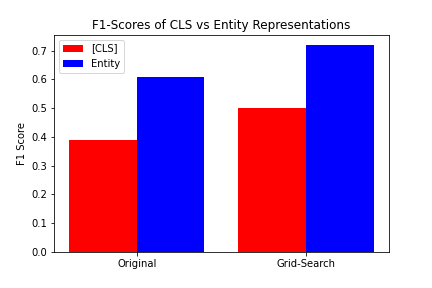
\includegraphics[width=10cm]{images/graph.png}
  \caption{Graph comparing the F1-Scores obtained from [CLS] and entity ([E1]/[E2]) representations before and after finding optimal parameters with grid search}
  \label{fig:search}
\end{figure}

The preference of a newton-cg solver over the initial saga solver used before could be due to the high dimensionality of the data, since newton-cg computes a hessian matrix from the objective function which is independent to the number of features. Conversely, the gradient computation for saga scales linearly with the number of features. It is worth noting that as a consequence of computing second derivatives for this dataset, the time taken to classify each sentence significantly increased. In addition, the newton-cg solver was incompatible with the L1 regularisation method, so the optimal method resulted in the same as the original model (L2). According to the results from grid search, using a higher value for the C parameter of grid search was preferred, indicating that providing more weight to the training data results in the detection of better patterns that can be applied to the test set.

It is possible that these values chosen by grid search aren't representative of the most optimal parameters that could be used for the model. This implementation of grid search was limited by both time constraints and computational resources, and the results were heavily dependent on the number of iterations required for each solver to converge. For the vast majority of solvers tested, the solutions were forced to complete before they had finished converging to a solution, meaning the results they returned may not have been entirely representative of the quality of the model. There was an attempt to reduce the effect of this during implementation by increasing the 'max\_iter' parameter from the default value (100) to 500 iterations. Increasing this further expended computational resources and couldn't be completed.

Now that the model has been optimised to fit the data, the results from each research question can be combined to create a model that theoretically has the most optimal performance. Obtaining the entity representation from sentences containing context and type and applying a dropout value of 0.5 results in the values displayed in figure \ref{fig:best}:

\begin{figure}[h]
\begin{center}
\begin{tabular}{||c c c c||} 
 \hline
 Embeddings & F1-Score & Precision & Recall \\ [0.5ex] 
 \hline\hline
 Training & 0.84 & 0.90 & 0.83 \\ 
 \hline
 Test & 0.73 & 0.79 & 0.70\\
 \hline
\end{tabular}
\end{center}
\caption{Evaluation Metrics for training and test sets for entity representations with context + type and dropout 0.5}
\label{fig:best}
\end{figure}

The results on the test set for sentences containing both context and type appear to be similar to the results for context and mention. It is possible that the model has reached a point where it is more at the mercy of the nature of the dataset, particularly for the none-type relation, and therefore no amount of optimisation can further improve the results without an attempt to balance the classes being inputted. Using the method of finding the Cartesian product over each potential relation contributed to this since the number of NONE-type relations vastly outnumbered the instances of other classes in the dataset. In the test set alone, there were around 9000 none-type instances, which is around 9 times the amount of instances compared to other labels with high instances.

In fact, upon further research, it was found that the removal of the NONE type relation altogether significantly improved the overall results of the model. It is likely that the inclusion of this measure provided more confusion about which trends to pick up on since there was more ambiguity in the structure of these none-type relations. There was then a concern that this newly discovered information would impact the overall trend of the resultant research questions, so each question was performed again without the None-type relations. It was found that the overall trends still remained the same despite this difference, however the F1 scores of all sentence representations had improved by a large margin. For example when extracting [CLS] representations from the first research question, the F1 score had increased from 39\% to 62\%. The entity representations experienced a fair increase from 61\% to 72\%. This still shows that entity representations in general performed better than [CLS] representations, and also emphasises that entity representations tend to be more resilient to extreme measures of class imbalance.

The results containing the F1 scores for every relation type is expressed within figure \ref{fig:results}. The relation with the highest F1 score is PART-OF, with an F1 score of 90\%, and the macro F1 score increased to 78\%. These scores indicate that the final model is very effective with the task of biomedical relation extraction, but there is still room for improvement which can be explored in the future.

\begin{figure}[h]
\centering
\begin{tabular}{||c c c c c||}
\textbf{Label} & \textbf{Precision} & \textbf{Recall} & \textbf{F1-score} & \textbf{Support} \\
ACTIVATOR & 0.55 & 0.69 & 0.61 & 243\\
AGONIST & 0.74 & 0.67 & 0.70 & 131\\
AGONIST-ACTIVATOR & 0.17 & 0.10 & 0.12 & 10\\
AGONIST-INHIBITOR & 0.00 & 0.00 & 0.00 & 2\\
ANTAGONIST & 0.80 & 0.89 & 0.84 & 215\\
DIRECT-REGULATOR & 0.72 & 0.76 & 0.74 & 442\\
INDIRECT-DOWNREGULATOR & 0.62 & 0.61 & 0.62 & 326\\
INDIRECT-UPREGULATOR & 0.62 & 0.63 & 0.63 & 301\\
INHIBITOR & 0.89 & 0.83 & 0.86 & 1148\\
\textbf{PART-OF} & \textbf{0.88} & \textbf{0.91} & \textbf{0.90} & \textbf{257}\\
PRODUCT-OF & 0.78 & 0.76 & 0.77 & 158\\
SUBSTRATE & 0.87 & 0.81 & 0.84 & 494\\
SUBSTRATE-PRODUCT OF & 0.33 & 0.33 & 0.33 & 3 \\
\end{tabular}
\caption{Table of final results}
\label{fig:results}
\end{figure}

%\begin{figure}[h]
%\begin{table}[h]
%\centering
%\begin{tabular}{||c c c c c||}
%\textbf{Label} & \textbf{Precision} & \textbf{Recall} & \textbf{F1-score} & \textbf{Support} \\
%\midrule
%ACTIVATOR & 0.27 & 0.53 & 0.36 & 243 \\
%AGONIST & 0.43 & 0.53 & 0.47 & 131 \\
%AGONIST-ACTIVATOR & 0.20 & 0.10 & 0.13 & 10 \\
%AGONIST-INHIBITOR & 0.00 & 0.00 & 0.00 & 2 \\
%ANTAGONIST & 0.60 & 0.77 & 0.68 & 215 \\
%DIRECT-REGULATOR & 0.30 & 0.67 & 0.42 & 442 \\
%INDIRECT-DOWNREGULATOR & 0.39 & 0.55 & 0.46 & 326 \\
%INDIRECT-UPREGULATOR & 0.34 & 0.54 & 0.42 & 301 \\
%INHIBITOR & 0.58 & 0.77 & 0.66 & 1148 \\
%NONE & 0.93 & 0.72 & 0.81 & 9666 \\
%PART-OF & 0.47 & 0.73 & 0.57 & 257 \\
%PRODUCT-OF & 0.34 & 0.60 & 0.43 & 158 \\
%SUBSTRATE & 0.39 & 0.66 & 0.49 & 494 \\
%SUBSTRATE-PRODUCT-OF & 0.00 & 0.00 & 0.00 & 3 \\
%\midrule
%\end{tabular}
%\end{table}
%\caption{}
%\label{fig:relations}
%\end{figure}

%==================================================================================================================================
\chapter{Conclusion}  
This research involved performing supervised biomedical relation extraction using a deep learning approach and investigated modelling different sentence inputs to encourage BERT to identify entities of interest and discover how they are related to one another. It then went on to elucidate which aspects of BERT's output best represent the input representations for BERT to observe which input was the most appropriate for the biomedical domain.

The results for the first research question demonstrated that using entity representations rather than [CLS] representations from BERT's output provides more information about the semantics of the entities being classified, It can be observed that this supervised relation extraction approach is only as effective as the quality and quantity of annotations provided for each class. If there is only a small number of annotations for one class, it is significantly less likely for the model to correctly predict sentences relating to that class.

The results for the second research question demonstrates that omitting entity mentions from the input but still providing some information about their type can provide superior results, compared to providing context and mention or just context. This follows on from the research of \cite{mask}, who concluded that specifying the type of the entity had a significant impact on the quality of the model. However, this implementation contradicted their results stating that including both context and mention provided the most optimal results. The best F1 score on the test set was 74\% compared to 61\% for entity markers and 64\% for just context. It is possible that within the biomedical domain, reducing the multi-token entities included within the input text provided succinct enough information that BERT was able to learn better patterns from it.

The third research question shows that the most effective level of dropout is similar for different sentence representations, with the best value for [CLS] representations being 0.6, and the best value for entity representations being 0.5. These values provide enough noise reduction to more accurately reflect trends for different relations without excessive obfuscation. However, it also highlighted the limitations of using logistic regression, since the metrics can be slightly unstable offer differing results for each run.

The discussion emphasises the importance of optimising logistic regression in order for it to be more effective at determining class boundaries during multi-class classification, and ensuring that the correct regularisation methods are being used on the data to prevent over-fitting to the training data. The findings suggest that using a newton-cg solver and increasing trust in the training data significantly increases the performance, at the expense of computational resources. It was also discovered that removing the none-type relation instances from the training and test sets removed ambiguity during training, and resulted in a 7\% increase in F1 score metrics across all relations.

The best F1 score for a specific relation was for PART-OF, with an F1 score 0f 90\%. The best overall F1 score on the test set was achieved by combining the optimal results obtained for each research question, which is 78\%. The resultant model is therefore relatively effective with the task of biomedical relation extraction.

\newpage
\section{Future Work}
Despite the attempt to mitigate class imbalance, it still had a significant impact on the overall quality of the model, with many estimations being for classes with the most instances in the training and test sets. Findings from the drugprot overview paper by \cite{overview} suggested that the best models utilised an ensemble of various models and enriched the encoding part of the system through external resources and data augmentation. The best results for the DrugProt task were obtained by \cite{humboldt}, who scored 79\% on the test set. Within their attempt, they found the best results by enriching the input text with descriptions of the chemicals involved in the relations and ensembled ten different models by taking the average F1 score. If this research were to be reattempted, more effort would be made to reduce class imbalance by performing more data augmentation and by looking more into adjustments that can be made to the model to provide it with more information about each entity and ensure that it can handle the high-dimensional input classes more effectively.



 \begin{figure}[htb]
    \centering
    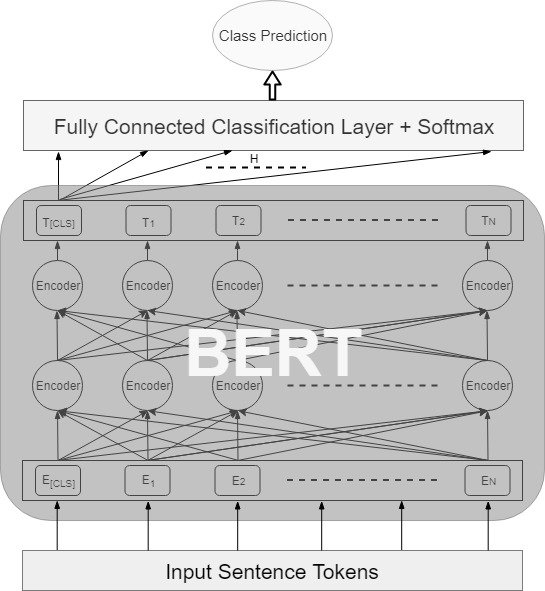
\includegraphics[width=10cm]{images/Fine-tune.jpg}
  \caption{Example of fine-tuning BERT architecture}
  \label{fig:fine}
\end{figure}

One potential aspect to explore would be to employ fine-tuning to produce more of an end-to-end system instead of feature extraction. Fine-tuning is the idea of creating an additional output layer to create models that can perform various tasks, including relation extraction and question answering, without having to perform substantial architecture modifications. Figure \ref{fig:fine} shows an example of this architecture. This has the added benefit of adjusting the feature weights at all system parts, including classification, rather than freezing the weights and inputting them into a separate classification model. \cite{tune} compared using fine-tuning and feature extraction on several proposed tasks, such as Named Entity Recognition, question answering and text classification. They discovered that when it came to using BERT, fine-tuning significantly outperformed feature extraction.

There are several limitations regarding supervised biomedical relation extraction. As much as it is incredibly effective to have high-quality annotations made by domain experts and explicit negative examples of relations, manually annotating these entities is still a very time-consuming process, and the results need to be better generalised. One way to mitigate this is to explore more generalised approaches to relation extraction, as mentioned within \cite{architectures}'s paper on 'Matching the blanks' (MTB). This introduces a new method that does not require pre-defined ontology or relation-labelled training data. It involves finding the inner product of relation statements with the entity names replaced with [BLANK] tags, with the idea that sentences with high inner products are likely semantically similar to those with low inner products. The fine-tuned BERT model can be combined with this MTB model, potentially producing improved results.


%==================================================================================================================================
%
% 
%==================================================================================================================================
%  APPENDICES  

%\begin{appendices}

%\chapter{Appendices}



%\end{appendices}

%==================================================================================================================================
%   BIBLIOGRAPHY   

% The bibliography style is abbrvnat
% The bibliography always appears last, after the appendices.

\bibliographystyle{abbrvnat}

\bibliography{l4proj}

\end{document}
